% !TEX root = ../thesis.tex
\section{Doplnění řečového korpusu o specifická data - vliv nových dat na kvalitu akustického modelu}
\label{chap:realisation:corpus}

Před samotným pořízením nahrávek promluv je nezbytné vybrat co možná nejvíce dvojic slov, které se liší významem a znělostí právě jednoho fonému.
Příkladem takovýchto slov může být dvojice slov \textit{kosa} + \textit{koza} nebo \textit{přibít} + \textit{připít}.
Pro tento účel byl vyvinut algoritmus výběru slov, který provede výběr dílčích kroků pomocí

\begin{enumerate}
  \item načtení dat (slovník a hledané párové fonémy);
  \item shluknutí všech slov vedoucích ke stejné fonetické transkripci;
  \item vytvoření všech možných kombinací dvojic slovních transkripcí;
  \item nalezení dvojic transkripcí, které se liší právě ve znělosti jednoho fonému\footnote{Algoritmus vzájemně porovná obě slova a najde rozdílné fonémy. Pokud tyto rozdíly odpovídají některé z dvojic párových fonémů, tak je dvojice přijata.};
  \item výběr dvojic slov na základě vybraných fonetických transkripcí.
\end{enumerate}

\noindent Jako slovník byl použit seznam slov s~fonetickými přepisy, které pocházejí z jazykového modelu obsahujícího 1,2 milionu slov.
Pomocí výše zmíněného algoritmu se podařilo nalézt $160$ párů slov lišících se znělostí právě jednoho fonému, celkem tedy $320$ slov.
Ke každému nalezenému slovu se následně vybrala minimálně jedna věta obsahující toto slovo (ale nikoli druhé slovo z dvojice).
Těchto vět je pak $418$. Příklad vybraných vět je uveden níže:

\begin{verbatim}
  Zkoušel jsem to několikrát, ale pokaždé padla kosa na kámen.
  Do basy nemusí, vlk žere, koza žije.
\end{verbatim}

Vybraná slova a věty se staly základem pro 2. etapu nahrávání.
Ta se uskutečnila během dvou sezení v~červenci roku 2016 se stejným řečníkem jako v~1. etapě.
Jde tedy o relativně velký časový odstup od 1. etapy.
Jednotlivá nahrávací sezení měla mezi sebou týdenní rozestup.
Oproti 1. etapě probíhalo nahrávání v~odhlučněné nahrávací komoře za pomocí profesionálního nahrávacího zařízení.
Studiový mikrofon byl od úst řečníka vzdálen přibližně 15 cm.
K nahrávání byl použit speciální software, který kontroloval, zda každá nahrávka splňuje určité parametry.
Každá akceptovaná nahrávka musela mít na svém začátku a konci minimálně $0,5\ s$ ticha a zároveň celá nahrávka nesměla být příliš tichá a zároveň přebuzená (kontrolováno pomocí energie).
Pokud nahrávka nesplňovala definované parametry, byla zamítnuta a řečník musel promluvu zopakovat.

Oproti 1. etapě nahrávání byla eliminována role anotátorů, v~důsledku mnohem širších možností nahrávacího softwaru.
% v~části \ref{chap:construction:corpus} je zmíněno, že je nezbytné provádět anotaci nahrávek, aby mohl být korpus kompletní. Samotná anotace je relativně zdlouhavý proces, a proto je dobré pořídit přesné promluvy vybraných slov a vět již v~průběhu nahrávání. K tomu slouží další z funkcí
Nahrávací software řečníkovi vždy ukáže text, který je potřeba vyslovit, a následně jej společně s~audio záznamem uloží.
K dispozici je tedy nahrávka a její \uv{přepis}.
Nicméně samotný řečník často může udělat chybu aniž by si toho všiml (např. záměnou podobných slov apod.).
Software ale žádným způsobem nekontroluje co je ve skutečnosti vysloveno, proto je nahrávání přítomen operátor, který poslouchá co bylo řečeno a v~případě potřeby zamítne nahrávku.
Řečník následně musí promluvu opakovat, dokud nahrávka neodpovídá požadovaným parametrům a zároveň není obsahově správně.

Na obr. \ref{fig:realisation:corpus:word} a \ref{fig:realisation:corpus:sentence} jsou ukázky audio záznamu slova \uv{kosa} a věty \uv{Zkoušel jsem to několikrát, ale pokaždé padla kosa na kámen.}.
Pokud se nahrávky porovnají s~nahrávkami získanými v~1. etapě (obr. \ref{fig:construction:el_speech}), je patrná vyšší kvalita nahrávek, zejména vyšší amplituda.
Ze zobrazených spektrogramů je zřejmé, že šum je přítomen v~menším množství a intenzitě než v~nahrávkách získaných v~průběhu 1. etapy.
Hlavní vliv na toto má studiový mikrofon, který není přilepen ke tváři řečníka, a tudíž nezaznamenává vibrace přenášené měkkou tkání.
Další rozdíl je vidět v~oblasti nižších frekvencích spektrogramu, ty jsou výraznější.
Přestože se jedná o stejného řečníka, zaznamenaná řeč nemá úplně identické parametry.
Jedním z důvodů bude nepochybně změna nahrávací aparatury a procesu nahrávání.
Nezanedbatelný vliv má i relativní nestálost parametrů EL řeči.
Ty jsou závislé na typu a pozici elektrolarynxu.
Ten se v~době mezi nahráváními navíc změnil, což v~konečném důsledku představuje asi hlavní důvod diference parametrů.

\begin{figure}[hbpt]
  \centering
  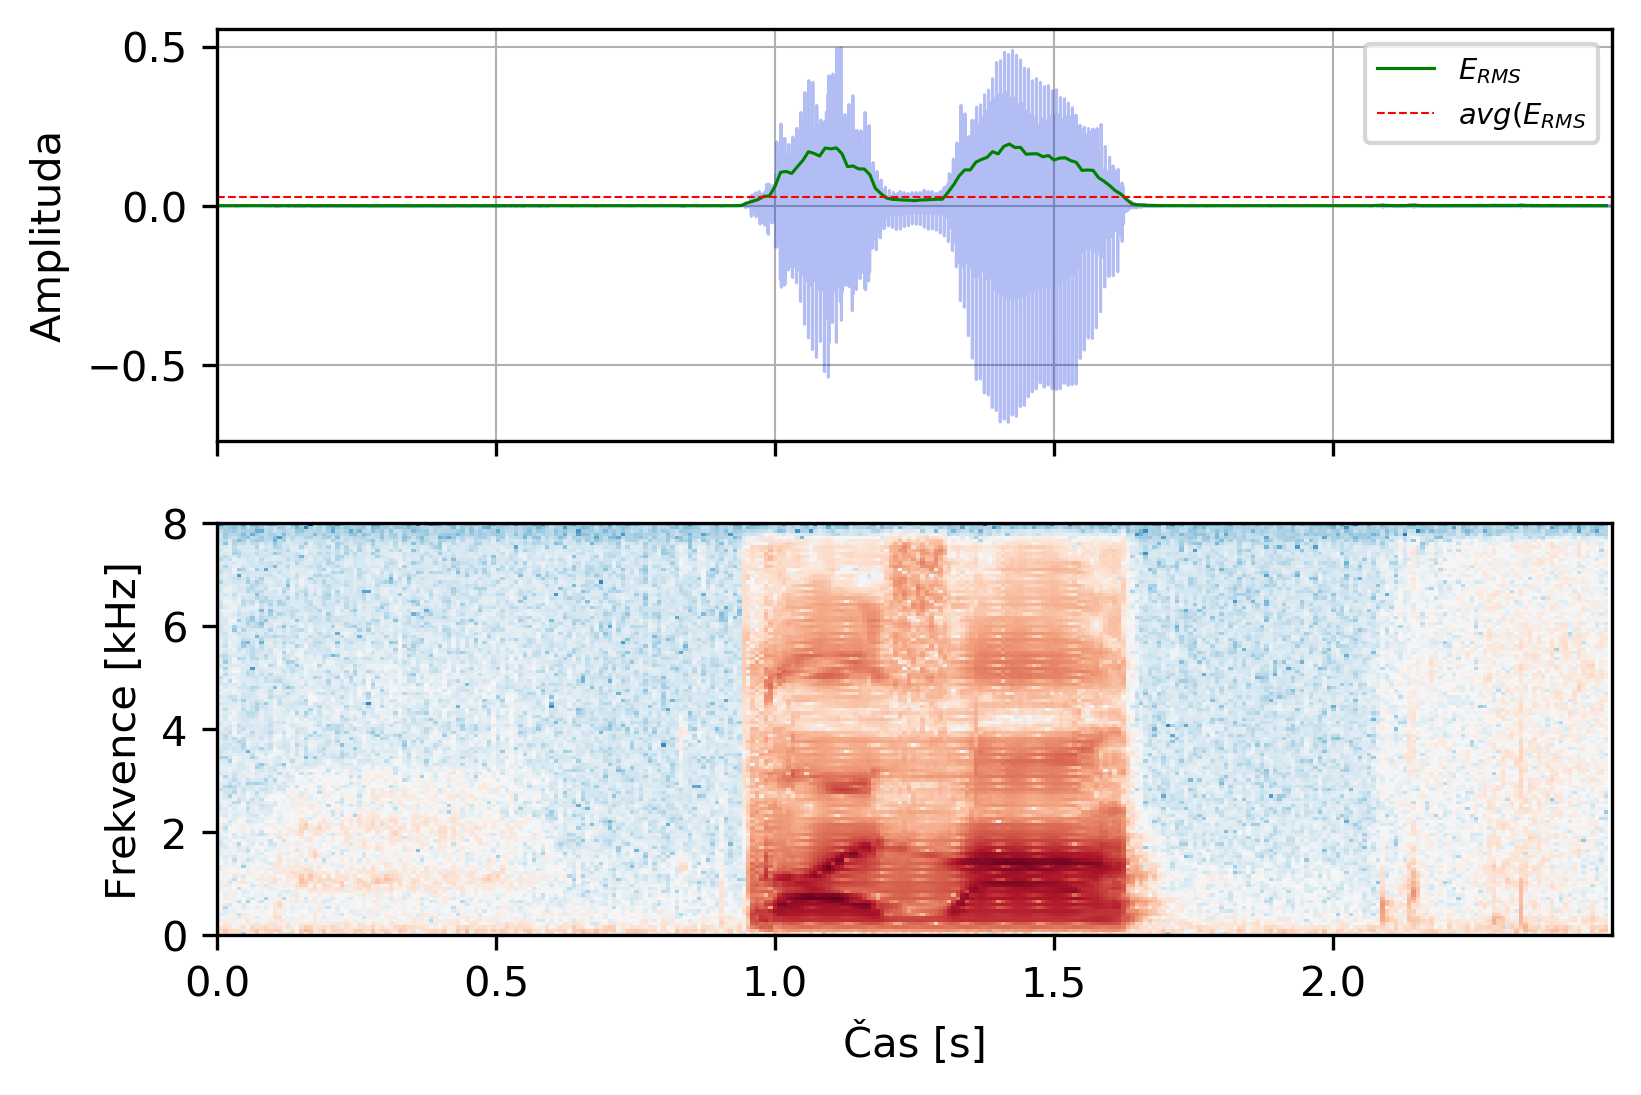
\includegraphics[width=0.9\textwidth]{./ch5-construction/img/energy_spec_word.png}
  \caption[Průběh a spektrogram slova \uv{kosa}.]{Průběh a spektrogram slova \uv{kosa} s~společně s~vyznačenou energií EL promluvy.}
  \label{fig:realisation:corpus:word}
\end{figure}

\begin{figure}[hbpt]
  \centering
  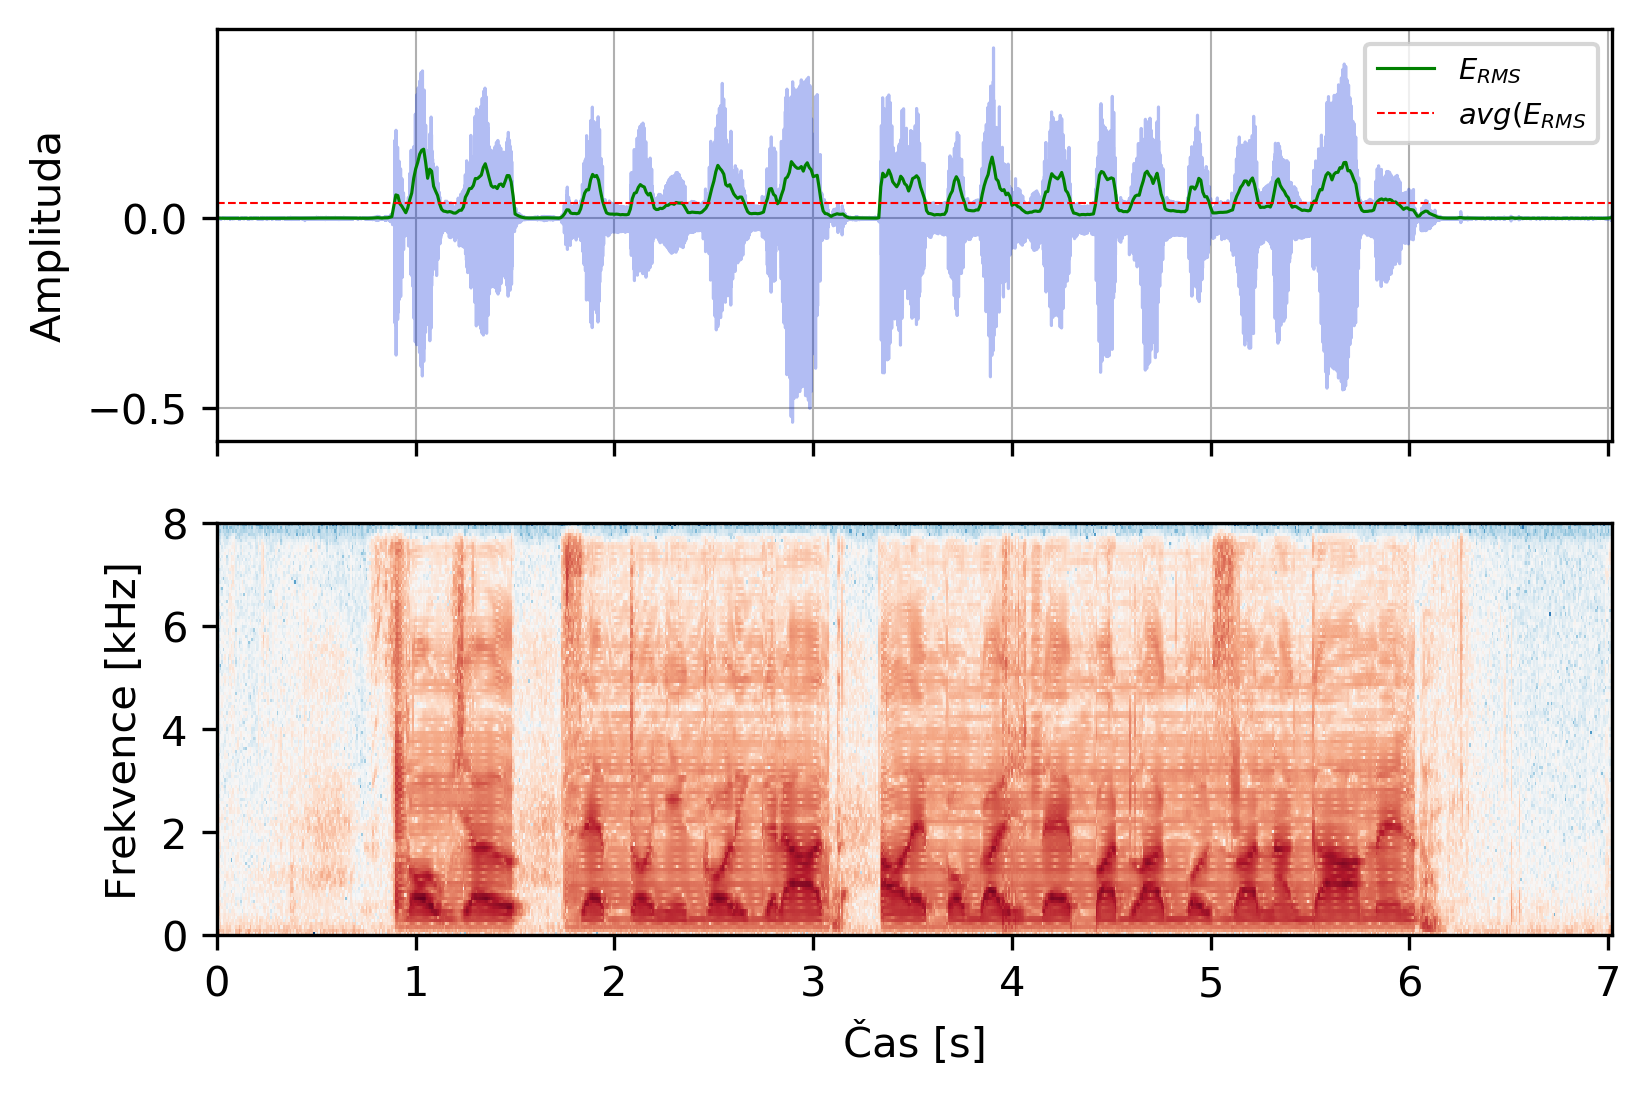
\includegraphics[width=0.9\textwidth]{./ch5-construction/img/energy_spec_sentence.png}
  \caption[Průběh a spektrogram promluvy obsahující slovo \uv{kosa}.]{Průběh a spektrogram promluvy obsahující slovo \uv{kosa} s~vyznačenou energií EL promluvy.}
  \label{fig:realisation:corpus:sentence}
\end{figure}

Tab. \ref{tab:realisation:corpus:recording} přibližuje souhrnné parametry nahrávek pořízených v~2. etapě nahrávání.
Celkem se podařilo získat přibližně 2 hodiny řeči (každá nahrávka obsahuje $0,5\ s$ ticha na začátku a konci).
Z toho přibližně jen $10~\%$ představují vybraná izolovaná slova.
Dohromady s~novými daty obsahuje korpus téměř $14$ hodin audio záznamů a jim odpovídajících přepisů.

\begin{table}[htpb]
  \centering
  \def\arraystretch{1.5}
  \pgfplotstabletypeset[
    col sep=comma,
    string type,
    columns/phase/.style={column name=Nahrávání, column type={l}},
    columns/length/.style={column name=Délka \textit{[HH:MM:SS]}, column type={r}},
    columns/words/.style={column name=Počet slov, column type={r}},
    columns/sentences/.style={column name=Počet vět, column type={r}},
    columns/files/.style={column name=Počet souborů, column type={r}},
    every head row/.style={
      after row={
        \cmidrule(r){1-1}
        \cmidrule(lr){2-2}
        \cmidrule(lr){3-3}
        \cmidrule(lr){4-4}
        \cmidrule(l){5-5}
      },
      before row={\toprule}},
    every last row/.style={
      after row={\bottomrule}
    },
  ]{./ch5-construction/tabs/0201-recording-stats.csv}
  \caption{Informace o korpusu nahrávek z 2. etapy nahrávání.}
  \label{tab:realisation:corpus:recording}
\end{table}

\subsection{Vliv nových dat na kvalitu modelů}
\label{chap:realisation:corpus:influence}

%Mezi lety 2012 a 2016 zaznamenalo rozpoznávání řeči překotný vývoj používaných technologií. Do té doby state-of-the-art modely stavěly na kombinaci HMM a \uv{gaussovských směsí} \textit{GMM}  U těchto modelů má každý HMM stav svou směs, viz obr. \ref{fig:realisation:corpus:hmm:gmm}. Pravděpodobnost přechodu mezi stavy HMM pak určují tyto směsi. Jejich parametry jsou získány na základě trénování. S příchodem open source frameworku Kaldi \cite{Kaldi2011} a rozmachem GPU výpočtů se začaly objevovat modely využívající hluboké neuronové sítě (DNN) .

%Rozpoznávání řeči je možné si představit sequence-to-sequence modely, tedy jako převod sekvence akustických parametrů do sekvence znaků/slov. Pro tento typ úloh se a priori hodí rekurentní neuronové sítě (RNN), ale jejich slabinou je enormní výpočetní náročnost i mimo trénovací fázi a také potřeba enormního množství dat, pokud má být vytvořen end-to-end\footnote{End-to-end systémem je ve valné většině případů myšlen systém, do kterého vstupuje audio framů a  vystupuje z něj sekvence znaků. Vývojář takového systému často nepoužívá parametrizované audio.} systém \cite{Hannun2014}. Vytvoření čistě RNN end-to-end ASR systému je tak nesmírně nákladné (data, HW, atd.). V~současné době se převážně využívá kombinace HMM modelu, který je také zástupcem rodiny sequence-to-sequence modelů, a DNN  Hlavním rozdílem oproti těm s~\textit{GMM} spočívá v~tom, že pro všechny HMM stavy se trénuje pouze jedna neuronová síť, pomocí které jsou určovány přechody mezi stavy, viz obr. \ref{fig:realisation:corpus:hmm:dnn}. Navíc tím, že tato neuronová síť určuje \uv{pouze} přechody mezi jednotlivými stavy HMM, tak může být řádově menší a jednodušší, než kdyby se jednalo o end-to-end model. Tím pádem je rychleji natrénovaná a je potřeba řádově méně dat.


% \begin{figure}[htpb]
%   \centering
%   \begin{subfigure}[b]{0.4\textwidth}
%     \includegraphics[width=\textwidth]{./ch5-construction/img/HMM-GMM.pdf}
%     \caption{HMM-GMM}
%     \label{fig:realisation:corpus:hmm:gmm}
%   \end{subfigure}
%   %
%   \begin{subfigure}[b]{0.4\textwidth}
%     \includegraphics[width=\textwidth]{./ch5-construction/img/HMM-DNN.pdf}
%     \caption{HMM-DNN}
%     \label{fig:realisation:corpus:hmm:dnn}
%   \end{subfigure}
%   \caption{Znázornění odlišného principu \textit{HMM-GMM} a \textit{HMM-DNN}.}
%   \label{fig:realisation:corpus:hmm}
% \end{figure}

% \subsubsection{Ověření přínosu nových dat}

Rozšíření korpusu umožňuje vytvoření nových modelů, pomocí kterých lze ověřit konzistenci a vliv nových dat na přesnost rozpoznávání.
Oproti baseline modelu jsou všechny následující modely vytvořeny ve frameworku Kaldi.
Ten se po roce 2015 stal standardem pro vytváření akustických modelů, protože je velmi flexibilní a umožňuje snadné přidávání nových typů akustických modelů \cite{Kaldi2011}.

%Oproti \ref{chap:realisation:analysis:experiment} je použit framework Kaldi, který se stal standardem pro vytváření akustických modelů. Samotný framework se skládá z velkého množství utilit, která každá plní určitý \uv{jednoduchý} úkol v~procesu vytváření a testování modelu. Kompletní proces vytváření modelu se tak sestává z postupného spouštění těchto utilit v~přesně definovaném pořadí. Autoři frameworku připravili nepřeberné množství skriptů, které slouží  k~vytvoření různých typů modelů. Všechny modely pro EL řeč vycházejí ze skriptů pro vytvoření akustických modelů z Wall Street Journal (WSJ) korpusu. Ten je nejčastěji požíván jako jakýsi benchmark ASR systémů. Skripty jsou jen drobně upraveny, aby výsledný model pracoval s~EL doménou.

Již při vytváření baseline modelu se ukázala lepší funkce DNN modelů.
Přestože vývoj výpočetních GPU postupuje závratnou rychlostí, tak natrénování HMM-DNN modelu je čásově náročnější než vytvoření HMM-GMM akustického modelu.
Navíc, jak bylo popsáno v~\ref{chap:asr:acoustic:DNN},  k~natrénování DNN modelu je potřeba zarovnání získané pomocí HMM-GMM modelu.
Proto je vhodné prvotní validaci nových dat provést na jednodušším modelu.

%Nicméně jak bylo popsáno v~\ref{chap:asr:acoustic:DNN}  k~natrénování modelu s~neuronovými sítěmi je potřeba zarovnání získané pomocí HMM-GMM modelu. Navíc natrénování HMM-DNN modelu je časově náročnější přestože vývoj výpočetních GPU postupuje závratnou rychlostí.

%Přestože DNN nahradily \textit{GMM} v~HMM, tak  k~jejich natrénování je nezbytné nejprve natrénovat \textit{HMM-GMM} model, který slouží  k~prvotnímu zarovnání (určení hranic jednotlivých fonémů v~rámci audio nahrávky). To slouží jako startovní bod pro neuronovou síť. Tím, že je trénována pouze jedna síť, tak je  k~dispozici řádově více dat\footnote{V případě \textit{HMM-GMM} má každý stav své \textit{GMM}, a tím pádem, čím více stavů, tím méně trénovacích dat pro každou směs.}  k~jejímu natrénování, na druhou stranu má tato síť mnohem více parametrů než všechny \textit{GMM} směsi dohromady a tak je potřeba dbát na velikost sítě. Nicméně pro standardní WSJ DNN (6 vrstev, každá s~1024, 2048 nebo 4096 neurony) je dat dostatek.

%Přestože vývoj výpočetních GPU postupuje závratnou rychlostí, tak natrénování standardního \textit{HMM-DNN} modelu trvá o poznání déle než \textit{HMM-GMM}. Pro ověření zda je možné vytvořit model ze všech dat, která jsou  k~dispozici, poslouží dobře i \textit{HMM-GMM} model, který stejně slouží jako startovní bod pro \textit{HMM-DNN}, tak by se vytvářel tak jako tak. Pokud tyto modely neposkytnou DNN  alespoň trochu \uv{dobré} počáteční podmínky, tak sofistikovanější DNN nemusí pomoci.

Proces vytvoření akustického modelu vychází z předpřipravených Kaldi trénovacích skriptů pro vytvoření modelu pomocí Wall Street Journal korpusu.
Tyto skripty jsou jen drobně upraveny tak, aby výsledný model mohl být natrénován z EL korpusu. Data jsou parametrizována pomocí PLP s~12 kepstrálními, delta a delta-delta koeficienty\footnote{V rámci úprav Kaldi skriptů se PLP parametrizace ukázala jako vhodnější pro EL řeč. Ověření proběhlo experimentálně. Byly vytvořeny dva identické HMM-GMM modely s~4096 stavy, ale každý byl natrénován na jinak parametrizovaných datech (MFCC a PLP). PLP model dosáhl o~$1,31~\%$ absolutně vyšší přesnost rozpoznávání.}. Nejprve je vytvořen monofónový model, který slouží jako iniciační model pro trifónové  modely, viz obr. \ref{fig:construction:results:baseline:hmm:training}.

%Tento monofónový model je speciální případ kontextově závislých modelů, bez levého a pravého (fonémového) kontextu. Následně jsou natrénovány trifónové modely. Stejně jako v~experimentech provedených v~části \ref{chap:realisation:analysis:experiment}, tak i zde jsou použity rozhodovací stromy, protože počet všech variant trifónů je příliš velký a dat nedostatek.

V části \ref{chap:construction:results} bylo popsáno rozdělení korpusu na trénovací a testovací sadu.
Po rozšíření korpusu je rozdělení dat z 1. etapy ponecháno a nová data  k~jednotlivým sadám přidána.
Všechny věty nahrané v~2. etapě jsou přidány do trénovací sady a všechna slova naopak do testovací sady.
Toto rozdělení vychází z impulzu pro rozšíření korpusu o specifická slova.
Ta tedy a priori mají sloužit  k~otestování nových modelů, a tedy i lepšímu porozumění problematice znělosti u EL řeči.

%Toto rozdělení je logické, protože důvodem rozšíření korpusu je snaha ověřit funkčnost ASR systémů na slovech, která mají rozdílný význam, ale liší se pouze znělostí jednoho fonému. Jelikož z výsledků v~části \ref{chap:realisation:analysis:reduction} vyplývá, že určité spektrum trifónů je možné reprezentovat pouze pomocí znělých variant, tak při použití nahraných slov bude teoreticky možné lépe prozkoumat tuto otázku.

Jazykový model je opět fonémový zerogramový.
Na kompletní testovací sadě bylo dosaženo přesnosti rozpoznávání $Acc_{p}^{GMM} = 54,96~\%$\footnote{Celková délka nahrávek v~testovací sadě složené z vět a slov činila $1h16m42s$.}.
V případě, že testovací sada obsahuje pouze nově nahraná slova, tak dokonce jen $Acc_{p}^{GMM} = 42,97~\%$\footnote{Celková délka nahrávek v~testovací sadě složené pouze slov činila $15m44s$.}.
To je významné zhoršení oproti výsledkům dosažených u baseline modelu ($Acc_{p}^{GMM} = 76,64~\%$).
Pro výpočet přesnosti rozpoznávání je opětovně využit vztah (\ref{eq:asr:decoding:acc}).

Jelikož došlo ke změně ASR frameworku je potřeba ověřit,že nevznikla chyba při vytváření akustického modelu.
K ověření je použit křížový test, kdy jsou pomocí stejného procesu natrénovány modely tvořené původními (1. etapa) a novými (2. etapa) daty a křížově otestovány na kompletní, původní a jen nové části testovací sady.
Trénovaný akustický model má stejné parametry jako v~předchozím případě.
Vstupem jsou PLP data s~12 kepstrálními, delta a delta-delta koeficienty, výsledný model může mít až 4096 stavů.
Výsledky testu jsou uvedeny v~tab. \ref{tab:realisation:verification:cross}.
Z té je jasně patrné, že trénovací proces proběhl správně a vině jsou tedy trénovací data.

%model;orig;new

\begin{table}[htpb]
  \centering
  \def\arraystretch{1.5}
  \pgfplotstabletypeset[
    col sep=semicolon,
    string type,
    columns/model/.style={column name=Model, column type={c}},
    columns/orig/.style={column name={1. etata}, column type={r}},
    columns/new/.style={column name={2. etapa}, column type={r}},
    every head row/.style={
      before row={
        \toprule & \multicolumn{2}{c}{$Acc_{p}\ [\%]$} \\
      },
      after row={
        \cmidrule(r){1-1}
        \cmidrule(l){2-3}
      }
    },
    every last row/.style={after row={\bottomrule}},
  ]{./ch5-construction/tabs/0202-cross_test.csv}
  \caption[Křížový test s~CMN.]{Křížový test modelů natrénovaných a otestovaných na datech z 1. a 2. etapy.}
  \label{tab:realisation:verification:cross}
\end{table}

% - 20161208_param -> porovnání n vs o, vzít hodnoty z toho
% - 20170111_together -> CMN  FULL výsledky na HMM, pak tam dat i výsledky z

\subsection{Eliminace vlivu kanálu}
\label{chap:realisation:corpus:elimination}

Z prezentovaných výsledků plyne, že nová data jsou příliš odlišná od původních a v~parametrickém prostoru jsou od nich příliš vzdálena.
Zároveň je těchto dat relativně malé množství na to, aby se mohly modely plně adaptovat.
Na zmíněný rozdíl v~datech je možné nahlížet jako na změnu kanálu.
Řečník je totiž stejný.
V předchozí části bylo zmíněno, že v~rámci 2. etapy došlo ke změně nahrávací procedury a elektrolarynxu.
Tím byl pozměněn kanál a řeč zaznamenaná v~2. etapě  má jiné parametry než ta původní z 1. etapy.
Mezi další vlivy, které mohou způsobit změnu kanálu, je např. prostředí, ve kterém je řeč produkována, nebo přítomnost šumu na pozadí.

K tomu, aby bylo možné použít všechna dostupná data, je tedy potřeba eliminovat vliv kanálu.
Standardně se  k~tomuto účelu používá Cepstral Mean Normalisation (CMN). Principem této metody je odstranění vlivu kanálu na základě střední hodnoty kepstrálních koeficientů.

Předpokládejme, že zaznamenaný signál $y[n]$ je možné popsat jako konvoluci promluvy a vlivu kanálu, tedy

\begin{equation}
  y\left[n\right] = x\left[n\right] \circledast h\left[n\right],
  \label{eq:experiments:normalization:convolution}
\end{equation}

\noindent kde $x\left[n\right]$ představuje vstupní signál, tedy řeč, a $h\left[n\right]$ odezvu kanálu na jednotkový impulz.
% Zaznamenaný signál je jejich již zmíněnou lineární konvolucí.
Ve frekvenční oblasti lze pak rovnici (\ref{eq:experiments:normalization:convolution}) zapsat ve tvaru

\begin{equation}
  Y\left[f\right] = X\left[f\right] \cdot H\left[f\right].
  \label{eq:experiments:normalization:convolution:reaq}
\end{equation}

\noindent Pro přechod do frekvenční oblasti byla využita FFT.
% Ve frekvenční oblasti se z konvoluce stává násobení.
Dalším krokem je převedení hodnot do kepstrální oblasti.
Pomocí logaritmu spektra, stejně jako v~případě MFCC parametrizace, viz \ref{chap:asr:parametrization:hearing}. V~kepstrální oblasti má vzorec (\ref{eq:experiments:normalization:convolution}), resp. (\ref{eq:experiments:normalization:convolution:reaq}) následující podobu

\begin{equation}
  Y\left[q\right] = \log\left(Y\left[f\right]\right) = \log\left(X\left[f\right] \cdot H\left[f\right]\right) = X\left[q\right] + H\left[q\right],
\end{equation}

\noindent kde $q$ představuje kepstrální koeficient.
V kepstrální oblasti je vliv kanálu aditivní složkou výsledného záznamu.
Problémem však je, že konkrétní hodnota vlivu kanálu je neznáma.
K dispozici je pouze výsledný ovlivněný signál.
Předpokládejme však, že vliv kanálu je stacionární\footnote{Jedná se sice o silný, ale logický předpoklad. Pokud se vztáhne na pořízený řečový korpus, tak v~rámci jedné etapy nahrávání je proces nahrávání neměnný, tzn. že je použita stejná aparatura a  k~nahrávání dochází vždy ve stejné místnosti.}.
Pak je možné každý frame nahrávky $i$ popsat pomocí vztahu

\begin{equation}
  Y_i\left[q\right] = H\left[q\right] + X_i\left[q\right],
\end{equation}

\noindent kde $Y_i\left[q\right]$ představuje $i$-tý frame kepstra $q$ nahrávky a $X_i\left[q\right]$ představuje $i$-tý frame kepstra $q$ neovlivněné řeči.
Z této rovnice je pak možné určit jeho střední hodnotu

\begin{equation}
  \frac{1}{N} \sum_i Y_i\left[q\right] = H\left[q\right] + \frac{1}{N} \sum_i X_i\left[q\right].
\end{equation}

\noindent Vliv kanálu je následně možné eliminovat odečtením této střední hodnoty kepstra $q$~od aktuální hodnoty kepstra $Y_i\left[q\right]$, konkrétně

\begin{align}
  R_i\left[q\right] &= Y_i\left[q\right] - \dfrac{1}{N}\sum_{j} Y_j\left[q\right] \nonumber  \\
  &= H\left[q\right] + X_i\left[q\right] - \left( H\left[q\right] + \frac{1}{N} \sum_j X_j\left[q\right] \right) \nonumber  \\
  &= X_i\left[q\right] - \frac{1}{N} \sum_j X_j\left[q\right].
  \label{eq:realisation:verification:cmn}
\end{align}

\noindent S pomocí rovnice (\ref{eq:realisation:verification:cmn}) je možné odfiltrovat vliv kanálu a teoreticky tak získat nezkreslený signál.
Otázkou je, přes jaký úsek počítat střední hodnotu.
Je možné ji počítat přes posuvné okénko fixní délky, přes jednotlivé věty/nahrávky, nebo dokonce přes všechny nahrávky konkrétní etapy.
Optimální úsek pro výpočet stř. hodnoty byl stanoven na základě provedených experimentů.

\subsubsection{Určení délky úseku pro výpočet CMN}

Ke stanovení vhodné délky úseku pro výpočet střední hodnoty kepstra $q$~zaznamenaného signálu byla využita stejná trénovací procedura, tj. byl
%K určení vhodné délky úseku pro výpočet střední hodnoty CMN byla použita stejná trénovací procedura jako v~předešlých experimentech s~novými daty.
trénován HMM-GMM model s~maximálně 4096 stavy, vstupní data byla parametrizována pomocí PLP.
% Na ně je aplikováno CMN počítáno z různé délky úseku.
Celkem jsou uvažovány dva experimenty, a to

\begin{itemize}
  \item CMN počítáno pro každou nahrávku,
  \item CMN počítáno pro celou etapu.
\end{itemize}

V tab. \ref{tab:realisation:verification:cmn:file} jsou uvedeny výsledky experimentu s~CMN počítaném přes jednotlivé nahrávky.
Z dosažených výsledků je patrné, že oproti výsledkům zaznamenaným v~tab. \ref{tab:realisation:verification:cross} je dosaženo určitého zlepšení, zvláště pro případy, kdy je model natrénován na datech z 1. etapy a otestován na datech z 2. etapy.
Výsledky však nejsou zdaleka tak dobré, jako v~případě trénování a testování modelu na datech ze stejné sady.
Významnou roli tu hraje fakt, že zejména nahrávky izolovaných slov jsou relativně krátké a vypočtené střední hodnoty, tak nabývají odlišných hodnot.

\begin{table}[htpb]
  \centering
  \def\arraystretch{1.5}
  \pgfplotstabletypeset[
    col sep=semicolon,
    string type,
    columns/model/.style={column name=Model, column type={c}},
    columns/orig/.style={column name={1. etata}, column type={r}},
    columns/new/.style={column name={2. etapa}, column type={r}},
    every head row/.style={
      before row={
        \toprule & \multicolumn{2}{c}{$Acc_{p}\ [\%]$} \\
      },
      after row={
        \cmidrule(r){1-1}
        \cmidrule(l){2-3}
      }
    },
    every last row/.style={after row={\bottomrule}},
  ]{./ch5-construction/tabs/0203-cmn_file.csv}
  \caption[Křížový test s~CMN přes jednotlivé věty.]{Křížový test modelů natrénovaných a otestovaných na datech z 1. a 2. etapy s~CMN  přes jednotlivé věty.}
  \label{tab:realisation:verification:cmn:file}
\end{table}

Další experiment byl proveden pro případ výpočtu CMN ze všech nahrávek konkrétní etapy.
V tab. \ref{tab:realisation:verification:cmn:full} je vidět markantní zlepšení výsledků.
Pokud byl model natrénován na datech z 1. etapy a otestován na datech z libovolné etapy, byly dosažené výsledky velmi podobné.
Nejhoršího výsledku bylo dosaženo pro případ, kdy byl model natrénován na datech z 2. etapy a otestován na těch z 1.
V tomto případě se projevil velký vliv relativně malého množství dat (pouhé 2 hodiny).
Pokud bylo CMN počítáno přes všechny nahrávky v~dané etapě, bylo dosaženo významného zlepšení a vliv kanálu byl v~podstatě eliminován.
Pro doplnění je nutno zmínit, že pokud byl model natrénován na celé množině všech trénovacích dat (1. a 2. etapa) a otestován pomocí kompletní testovací sady, tak byla dosažena přesnost rozpoznávání fonémovým zerogramovým jazykovým modelem rovna $Acc_{p} = 77,69~\%$.

%Tento výsledek je přibližující se hodnotám dosaženým v~prvotních experimentech v~části \ref{chap:realisation:analysis:experiment}.

\begin{table}[htpb]
  \centering
  \def\arraystretch{1.5}
  \pgfplotstabletypeset[
    col sep=semicolon,
    string type,
    columns/model/.style={column name=Model, column type={c}},
    columns/orig/.style={column name={1. etata}, column type={r}},
    columns/new/.style={column name={2. etapa}, column type={r}},
    every head row/.style={
      before row={
        \toprule & \multicolumn{2}{c}{$Acc_{p}\ [\%]$} \\
      },
      after row={
        \cmidrule(r){1-1}
        \cmidrule(l){2-3}
      }
    },
    every last row/.style={after row={\bottomrule}},
  ]{./ch5-construction/tabs/0204-cmn_full.csv}
  \caption[Křížový test s~CMN přes všechny nahrávky]{Křížový test modelů natrénovaných a otestovaných na datech z 1. a 2. etapy s~CMN  přes všechny nahrávky v~etapě.}
  \label{tab:realisation:verification:cmn:full}
\end{table}

Z výsledků v~tab. \ref{tab:realisation:verification:cmn:file} plyne, že pokud by se CMN počítalo přes posuvné okénko fixní délky, tak by dosažené výsledky nebylo možné považovat za dobré.
To se i experimentálně potvrdilo, protože výsledná přesnost rozpoznávání dosáhla hodnoty $Acc_{p} = 56,51~\%$ na kompletní trénovací i testovací sadě.
Samotný framework Kaldi umožňuje aplikování CMVN, což je Cepstral mean and variance normalization.
Jedná se o upravenou rovnici (\ref{eq:realisation:verification:cmn}), kde je kromě střední hodnoty počítána i variance.
Kaldi CMVN je počítáno přes okénko fixní délky a výsledná přesnost rozpoznávání HMM-GMM modelu s~CMVN dosáhla hodnoty $Acc_{p} = 76,15~\%$ na kompletní trénovací a testovací sadě.
Tento výsledek je srovnatelný s~modelem využívajícím výpočet CMN přes všechny nahrávky v~dané etapě.

\subsubsection{Výsledky modelů po eliminaci vlivu kanálu}

Aplikací CMN dosáhl HMM-GMM model srovnatelných výsledků s~výsledky dosaženými v~části \ref{chap:construction:results:baseline}.
Dalším krokem bylo natrénování HMM-DNN modelu.
%Po zjištění vhodného nastavení CMN, je dalším krokem natrénování neuronové sítě. V~předchozím textu bylo zmíněno, že neuronová síť jako počáteční podmínky používá zarovnání získané pomocí \textit{GMM}  To je získáno díky natrénovaným modelům s~CMN  přes všechny nahrávky.
Trénovaná neuronová FF síť měla 5 skrytých vrstev, výstupní vrstva byla typu softmax s~dimenzí rovnou počtu HMM stavů.
Postupně byla natrénována síť s~1024, 2048 a 4096 neurony v~každé skryté vrstvě.
Vstupní data byla parametrizována pomocí PLP s~12 kepstrálními, delta a delta-delta koeficienty a CMN počítané ze všech nahrávek dané etapy.
Byl využit fonémový zerogramový model, který minimalizoval vliv jazykového modelu na přesnost rozpoznávání.
Jazykový model je fonémový zerogramový tak, aby byl co nejvíce amplifikován vliv akustického modelu.
V tab. \ref{tab:realisation:verification:dnn} jsou zapsány dosažené výsledky všech natrénovaných variant.
Nejvyšší přesnosti dosáhl model s~4096 neurony v~každé vrstvě, ale rozdíl od ostatních variant s~menším počtem neuronů v~každé vrstvě nebyl významný.
Nejlepší HMM-DNN model dosáhl $Acc_{p} = 84,66~\%$.
To je zlepšení o~$6,97~\%$ absolutně oproti HMM-GMM na kompletní testovací sadě.

\begin{table}[htpb]
  \centering
  \def\arraystretch{1.5}
  \pgfplotstabletypeset[
    col sep=semicolon,
    string type,
    columns/neurons/.style={column name={Počet neuronů}, column type={c}},
    columns/accuracy/.style={column name={$Acc_{p}\ [\%]$}, column type={r}},
    every head row/.style={
      before row={\toprule},
      after row={
        \cmidrule(r){1-1}
        \cmidrule(l){2-2}
        % \midrule
      }
    },
    every last row/.style={after row={\bottomrule}},
  ]{./ch5-construction/tabs/0205-dnn.csv}
  \caption[Přesnost neuronové sítě s~monofónovým zerogramovým LM.]{Dosažená přesnost neuronové sítě s~monofónovým zerogramovým jazykovým modelem.}
  \label{tab:realisation:verification:dnn}
\end{table}
